\documentclass[12pt]{article}
\usepackage[margin=1in]{geometry}
\usepackage{ifpdf}
\usepackage{mla}
\usepackage{booktabs}
\usepackage{mathtools}

\usepackage{caption}
\captionsetup{labelsep=period}
\renewcommand{\figurename}{Fig.}

\usepackage[normalem]{ulem}

% Widow and orphan penalty.
\widowpenalty=10000
\clubpenalty=10000

\begin{document}
\begin{mla}{Colby}{Goettel}{Reed}{English 312}{21 March 2014}{Telecommunication Monopolies and Broadband Infrastructure}

% Intro, contract: WATCO the merger on BI?
This year, Comcast announced that it will be buying Time Warner Cable for a staggering \$45.2BN, all-stock. This merger between the two largest telecommunications companies in the United States will create a monopoly similar to AT\&T before its dissolution. These corporations are notorious for their poor customer service and lack of commitment to providing quality infrastructure and this merger will only further delay the building of proper broadband infrastructure in the United States. Some argue that this merger will not affect broadband infrastructure, only cable television. This paper will look at the effects the Comcast-Time Warner Cable merger will have on US broadband infrastructure.

% B: infrastructure
Fiber optic communication is the future of broadband. A single strand of single-mode glass fiber has a theoretical maximum bandwidth of 10\,Gbps for every person in the world. In other words, one strand of fiber can provide Gigabit Internet for every person ``on this planet and [nine] other planets the same size'' (Lunt).$^1$ Glass is primarily made of silicon dioxide~--- silicon rust. Once it's laid it doesn't go bad or deteriorate. The only pieces that need upgrading are the end connections~--- in a horribly simplified way, turning the light on and off. For this reason, when cities perform routine maintenance on roads and underground pipes, they need to bury fiber optic cable. Burying cables, as a rule of thumb, costs ten times as much as running cables overhead. Laying unused, or dark fiber is the cheapest route to installing infrastructure.

Other countries have already done this to a great extent. Paris laid fiber citywide over a decade ago. South Korea currently offers the best broadband Internet in the world. They offer Gigabit Internet for a measly \$25/mo on average. Google Fiber, currently hailed as the savior of Internet service, offers the same bandwidth for \$70/mo! As of Q4 2012, the United states was in 8th place for Internet speed (see table~\ref{table:connection-speed} and figure~\ref{figure:broadband-speeds}), trailing behind countries like Latvia and the Czech Republic. The bathroom light switches in Latvia are on the outside of the bathroom and they have better Internet than the US.

\begin{minipage}{\linewidth}
    \captionof{table}{Average Measured Connection Speed by Country/Region}\label{table:connection-speed}
    \begin{tabular}{llccc}
        \toprule
        ~  & Country/Region & Q4`12 Avg. Mbps & QoQ Change & YoY Change \\
        \midrule
        -  & Global         & 2.9  & 5.0\%  & 25\% \\
        1  & South Korea    & 14.0 & -4.8\% & -13\% \\
        2  & Japan          & 10.8 & 2.7\%  & 19\% \\
        3  & Hong Kong      & 9.3  & 3.4\%  & 5.4\% \\
        4  & Latvia         & 8.9  & 2.3\%  & 20\% \\
        5  & Switzerland    & 8.7  & 0.5\%  & 20\% \\
        6  & Netherlands    & 8.6  & 0.1\%  & 3.3\% \\
        7  & Czech Republic & 8.1  & 7.0\%  & 21\% \\
        8  & United States  & 7.4  & 2.3\%  & 28\% \\
        9  & Sweden         & 7.3  & 7.4\%  & 29\% \\
        10 & Finland        & 7.1  & 4.3\%  & 20\% \\
        \bottomrule
    \end{tabular}\par
    \bigskip
    Source: ``2013 Internet Statistics.'' \textit{Ispreview.co.uk}. N.p., 2013. Web.\bigskip
\end{minipage}

\begin{figure}
    \captionbox{Fixed (wired)-broadband subscriptions by speed, selected economies, 2010. Source: ``Fixed (wired)-broadband Subscriptions by Speed, Selected Economies, 2010.'' \textit{Ispreview.co.uk}. N.p., 2010. Web.\label{figure:broadband-speeds}}{%
        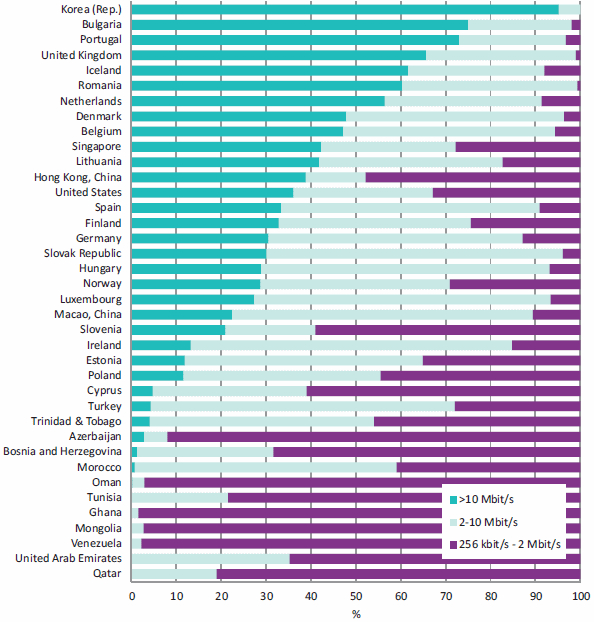
\includegraphics[bb = 0 0 594 622, scale=0.7]{broadband-speeds.jpg}%
    }
\end{figure}

% A: merger and monopoly history
The Comcast-Time Warner Cable merger still needs regulatory approval, but the cards seem to be stacked in its favor. Especially because Congress doesn't see this as an antitrust issue. Politico recently reported that 15/18 members of the Senate Judiciary Committee and 32/39 members of the House Judiciary Committee have received a donation from Comcast. This is legal bribery. This will ensure that Comcast will have its way throughout the hearings (Romm). Incredulously, Comcast has spoken up about this bribery saying that it is simply them being involved in the political process (Sottek). They have brazenly committed bribery and have brazenly dismissed their actions as natural, regular, part of the political process.

Up until the early 1980s, AT\&T controlled a monopoly on telecommunications in the United States known as Bell Systems, or Ma Bell. A government mandate on 08 January 1982 ordered the breakup of this monopoly. Once effected, this breakup allowed for long-distance telephone competition from Sprint and MCI. This competition lowered prices and provided better service for customers. The only downside of this monopoly breakup was the destruction of Bell Laboratories where most of the current hardware in use today (e.g., semi-conductors) was invented. This destruction cost the US their leading place in the Information Age. But the breakup was ultimately what the US needed for competition to push the telecommunications industry into the 21st century.

Unfortunately, since the breakup of Ma Bell, the Baby Bells (the companies created from the breakup) have reacquired most of their original strongholds. In fact, AT\&T's post-breakup ventured failed and it was acquired by one of the Baby Bells, SBC Communications, and renamed AT\&T Inc. They are now the second largest mobile company and largest landline company in the United States. They have acquired eleven of the original twenty-two Baby Bells. Since 1989, AT\&T has donated over \$56MM to political campaigns (Organizations) and more than \$130MM to lobbying (Kang). They have laid a pattern for Comcast to follow: monopoly and political bribery. This subversive behavior goes against what is best for customers and the future of telecommunication in America.

% C: tight regulations that don't allow for advancement
% A->C: merger's effects on regulations
The past decade of broadband infrastructure in Utah illustrates a great example of what happens to competition when monopolies exist. In the mid-2000s, seventeen Utah cities joined forces to provide quality fiber infrastructure to their residents. Their consortium is called the Utah Telecommunication Open Infrastructure Agency, or Utopia. The cities laid fiber optic cable and currently provide service to over 11,000 subscribers. Comcast didn't like the competition and paid off the Utah legislature to make it legal for cities to lay infrastructure, but illegal for them to advertise their service (Ekstrom).$^2$

Provo announced last year that Google Fiber would be buying their existing fiber infrastructure. This deal cost a grand total of \$1. Provo tried to sell for almost \$300MM, but Google said that they would pay \$1, nothing more, but would improve the existing infrastructure with almost \$500MM of work. This deal ended the city and its citizens from having to pay further taxes to pay off the infrastructure and will greatly improve the infrastructure in Provo (Richards). Unknown to most, Utopia actually provides better and cheaper service than Google Fiber. But they're not allowed to advertise it because Comcast paid off the legislature to make this illegal.

Fortunately, because Google Fiber is coming to Provo and improving infrastructure, they have forced Comcast to improve their service or be left in the dust. Comcast has since been going to existing customers and giving them free cable television and 50~Mbps Internet. The disgusting thing is that they have had the infrastructure in place for years to offer this kind of service, but didn't because there was no competition. Why the hell should any of their customers remain faithful to a company that has swindled them for years? This level of service is where backwater America should be right now, not large US cities (Venezia).

% C->B: regulations' effects on BI
% talk about KC, Google Fiber, and Comcast's effect there
% make sure it's explicit that this will limit both the current infrastructure (for money) as well as the future infrastructure
In Kansas City, the debut location for Google Fiber, Comcast along with Time Warner Cable and Cox are lobbying to create legislation that will deny cities the ability to build additional broadband infrastructure (Brodkin). The relevant part of their recent bill states:
\begin{mlaquote}
    Except with regard to unserved areas, a municipality may not, directly or indirectly:
    
    \begin{enumerate}
        \item Offer or provide to one or more subscribers, video, telecommunications, or broadband service; or
        \item purchase, lease, construct, maintain, or operate any facility for the purpose of enabling a private business or entity to offer, provide, carry, or deliver video, telecommunications, or broadband service to one or more subscribers.
    \end{enumerate}
\end{mlaquote}
This move would not only limit the current infrastructure, but block future construction and maintenance. A move like this will allow the existing ISPs to increase prices without providing additional services, just as they've done nationwide for years.

% procatalepsis
Many people have argued that this deal is about cable television and has nothing to do with the Internet. This couldn't be further from the truth. Cable television is mostly out the door. The only real foothold that cable television currently has is sports and reality TV. Everything else can be found online through streaming services. However, cable television won't fully die until the current generation dies. But nothing about this merger has to do with cable television. It's all about the Internet. According to tech pundit Paul Venezia, this merger ``is about controlling the content and delivery of Internet-based communication and entertainment'' (Venezia).

If corporations can control the Internet, its content and delivery, they will hold all of the cards in their hand. They will continue to not build out infrastructure and increase prices. They will extort their customers until they are forced, by competition, to improve. Competition is essential to the growth of the Internet and the stimulation of true innovation. This dearth of competition has been around for the recent history of the Internet. Again, from Venezia, ``[t]he massive advancement we saw in the first 10 years of our Internet consciousness is being destroyed by the deregulation and lobbying of the past nine'' (Venezia).

Others argue that Google presents a clear competition to Comcast and other area-monopolies. Unfortunately, all of the great effect that Google Fiber is having on broadband infrastructure is only happening in three cities nationwide. Three. Google is currently exploring an additional thirty-four cities, but their domain pales in comparison to the almighty power that Comcast and Time Warner Cable hold.

% A->B (conclusion): merger's effects on BI
Historically, Comcast and Time Warner Cable have both provided terrible service and infrastructure. They've already shown that they have the infrastructure in place to provide quality bandwidth, but don't because there is no incentive. They raise prices, provide terrible customer service, and pay off the legislature to get their way. Legislation has been passed in Utah and is currently underway in Kansas to further stymie broadband infrastructure and competition. Enough is enough. Tight regulations do not allow for advancement. The United States has poorer Internet than Romania and it's because of companies like Comcast and Time Warner Cable.

\newpage
\begin{center}
    Notes
\end{center}
\ \ \ \ \ 1. The Shannon--Hartley theorem, $C=B\log_2\left(1+\frac{S}{N}\right)$, is used to calculate the theoretical maximum of a communication medium. From Professor Lunt:
\begin{mlaquote}
    But I have also done the calculations myself, using Shannon's Law, and (as I showed in class) a single strand of single-mode fiber (not multi-mode) has enough bandwidth to allow for 10~Gbps for every person on the planet, or 1~Gbps for everyone on this planet and 9 other planets the same size.''
\end{mlaquote}

Mathematically, this is computed as follows. Let B represent the bandwidth of a channel and $\frac{S}{N}$ the signal-to-noise ration. Thus, using rough numbers:
\begin{align*}
    C&=B\log_2\left(1+\frac{S}{N}\right) \\
     &=4700~\text{MHz}\cdot\log_2\left(1+14~\text{dB}\right) \\
     &=4700000000~\text{Hz}\cdot\log_2(26.11886~\text{W}) \\
     &\approx2.2118\times10^{10}
\end{align*}

{\noindent\ \ \ \ \ 2. From Associate Professor Ekstrom regarding the role that Comcast played in disrupting Utah's fiber infrastructure and any possible sources to check:}
\begin{mlaquote}
    ``Obviously the legislature would argue that `cities shouldn't compete with private industry' [because] protected monopolies don't like competition.

    You would have to follow the money in the 2000--2005 period to see it. No reporter cared enough to document it. Most of the reporting has been iProvo and Utopia are dumb ideas that got the cities into debt, not why is Utah valley booming right now?

    Short answer, I don't know of any analysis of the political implications of the legal environment.''
\end{mlaquote}

{\noindent\ \ \ \ \ 3. Enthymeme: ``The Comcast-Time Warner Cable merger stymies US broadband infrastructure because it creates tight regulations that don't allow for advancement.''}

\begin{workscited}
    \bibent Brodkin, Jon. ``Cable Lobby Will `tweak' Bill Banning Municipal Broadband in Kansas.'' \textit{Ars Technica}. N.p., 31 Jan. 2014. Web. 31 Jan. 2014.
    
    \bibent Ibid. ``Who Wants Competition? Big Cable Tries Outlawing Municipal Broadband in Kansas.'' \textit{Ars Technica}. N.p., 31 Jan. 2014. Web. 31 Jan. 2014.
    
    \bibent Kang, Cecilia, and Jia Lynn Yang. ``How AT\&T Fumbled Its \$39 Billion Bid to Acquire T-Mobile.'' \textit{Washington Post}. The Washington Post, 11 Dec. 2011. Web. 21 Mar. 2014.
    
    \bibent Kessler, Andy. ``Why Super-Fast Internet Is Coming Super Slowly.'' \textit{The Wall Street Journal}. Dow Jones \& Company, 23 Feb. 2014. Web. 23 Feb. 2014.
    
    \bibent ``Organizations.'' \textit{Opensecrets RSS}. N.p., n.d. Web. 21 Mar. 2014.
    
    \bibent ``Question on Multi-mode Glass Fiber.'' Message to Professor Barry M.\ Lunt. 19 Mar.\ 2014. E-mail.
    
    \bibent ``Question on Utopia.'' Message to Associate Professor Joseph J.\ Ekstrom. 19 Mar.\ 2014. E-mail.
    
    \bibent Richards, John. ``Google Fiber.'' Jr./Sr.\ Seminar. 260~CTB, Provo. 30 January 2014. Seminar.
    
    \bibent Romm, Tony. ``Comcast Spreads Cash Wide on Capitol Hill.'' \textit{Politico.com}. N.p., 9 Mar. 2014. Web. 12 Mar. 2014.
    
    \bibent Sottek, T. C. ``There's one thing Republicans and Democrats can agree on: taking money from Comcast.'' The Verge. N.p., 10 Mar. 2014. Web. 10 Mar. 2014.
    
    \bibent Venezia, Paul. ``The Broadband Barbarians Will Soon Control the Gates.'' \textit{InfoWorld}. N.p., 24 Feb. 2014. Web. 24 Feb. 2014.
\end{workscited}

\end{mla}
\end{document}

A: merger
v1: stymies
B: BI b/c
A': the merger
v2: creates
C: tight regulations that don't allow for advancement
